\chapter{Appendix for Chapter~\ref{chap: linear}}
\section{Convexity}

\propconvex*
\begin{proof}[Proof of Proposition~\ref{prop: convexity} on page~\pageref{prop: convexity}]
  From Notation~\ref{not: scores}, threshold~$t_0$ is just a maximum from vector~$\bm{s}^-$ of scores of all negative samples.  Since maximum is a convex function, threshold~$t$ is a convex function of weights~$\bm{w}.$ Moreover, it is easy to show that the quantile~$t_1$ is not convex. Due to~\cite{lapin2015top}, the mean of the~$K$ highest values of a vector is a convex function. Therefore, threshold~$t_2$ is a convex function  of weights~$\bm{w}.$ It remains to analyze threshold~$t_3.$ Let us define function~$g$ as follows
  \begin{equation*}
    g(\bm{w},t) := \frac{1}{\nall} \sum_{i \in \I} l(\bm{w}^{\top} \bm{x}_i - t) - \tau.
  \end{equation*}
  where we set~$\vartheta = 1$ for simplicity. Then~$t_3$ is defined via an implicit equation~$g(\bm{w},t) = 0.$ Since~$l$ is convex, we immediately obtain that~$g$ is jointly convex in both variables.
  
  To show the convexity, consider~$\bm{w}, \; \tilde{\bm{w}} \in \R^d$ and the corresponding thresholds~$t = t_3(\bm{w})$,~$\tilde{t} = t_3(\tilde{\bm{w}})$. Then for any~$\lambda\in[0,1],$ we have 
  \begin{equation}\label{eq:proof_conv1}
    g\Brac{\lambda \bm{w} + (1 - \lambda)\tilde{\bm{w}}, \;\lambda t + (1 - \lambda)\tilde{t}}
    \leq \lambda g(\bm{w}, t) + (1 - \lambda) g(\tilde{\bm{w}}, \tilde{t}) = 0.
  \end{equation}
  The inequality follows from the convexity of~$g$  and the equality from~$g(\bm{w}, t) = g(\tilde{\bm{w}}, \tilde{t}) = 0,$ which holds due to the definition of~$t_3.$ From the definition of~$t_3,$ we also have
  \begin{equation}\label{eq:proof_conv2}
    g(\lambda\bm{w} + (1-\lambda)\tilde{\bm{w}}, \; t_3(\lambda\bm{w} + (1-\lambda)\tilde{\bm{w}})) = 0.
  \end{equation}
  Since~$g$ is non-increasing in the second variable, from~\eqref{eq:proof_conv1} and~\eqref{eq:proof_conv2} we deduce
  \begin{equation*}
    t_3(\lambda\bm{w} + (1-\lambda)\tilde{\bm{w}})
    \leq \lambda t + (1-\lambda)\tilde{t}
    =   \lambda t_3(\bm{w})+(1-\lambda) t_3(\tilde{\bm{w}}),
  \end{equation*}
  which implies that function~$\bm{w}\mapsto t_3(\bm{w})$ is convex.
\end{proof}

\thmconvex*
\begin{proof}[Proof of Theorem~\ref{thm: convexity} on page~\pageref{thm: convexity}]
  Due to the definition~\eqref{eq: confusion counts surrogate}, the objective function~$L$ equals to
  \begin{equation*}
    L(\bm{w}) = \fns(\bm{s}, t(\bm{w})) = \sum_{i \in \Ipos} l \Brac{t(\bm{w}) - \bm{w}^{\top} \bm{x}_i}.
  \end{equation*}
  Here we write~$t(\bm{w})$ to stress the dependence of~$t$ on~$\bm{w}$. Since~$\bm{w}\mapsto t(\bm{w})$ is a convex function, we also have that~$\bm{w} \mapsto t(\bm{w}) - \bm{w}^{\top} \bm{x}$ is a convex function. From its definition, the surrogate function~$l$ is convex and non-decreasing.  Since the composition of a convex function with a non-decreasing convex function is a convex function, this finishes the proof.
\end{proof}

\section{Differentiability}

\derivative* 
\begin{proof}[Proof of Theorem~\ref{thm: differentiability} on page~\pageref{thm: differentiability}]
  The non-differentiability of~$t_0,$~$t_1$ and~$t_2$ happens whenever the threshold value is achieved at two different scores. The result for~$t_3$ follows directly from the implicit function theorem. 
\end{proof}

\newpage

\section{Stability}\label{app: stability}

\degeneratebehavior*

Additionally to the assumptions from Example~\ref{ex: degenerate behaviour}, we consider the hinge loss function and no regularization for all formulations from Table~\ref{tab: summary formulations}. We also assume that~$n$ is large, and the outlier may be ignored for the computation of thresholds that require a large number of points.

\paragraph*{\TopPush formulation~\eqref{eq: toppush surrogate}:}
\begin{itemize}
  \item For~$\bm{w}_0 = (0,0)^{\top},$  all scores are equal to 0. Since the threshold~$t$ is the largest negative score, it also equals 0. Consequently, the value of the objective function is
  \begin{equation*}
    L(\bm{w}_0)
      = \frac{1}{\npos} \sum_{i \in \Ipos} \max\Brac[c]{0, \; 1 + (0 - 0)}
      = 1.
  \end{equation*}
  \item For~$\bm{w}_1 = (1,0)^{\top},$ the largest negative score equals~$2;$ therefore~$t = 2.$ Then, the value of the objective function is
  \begin{equation*}
    L(\bm{w}_1)
      \approx \int_{0}^{1} \max\Brac[c]{0, \; 1 + (2 - s_i)}
      = \int_{0}^{1} \Brac{3 - s} \dd{s}
      = \frac{5}{2},
  \end{equation*}
  where we can remove the~$\max$ operator since all positive samples are uniformly distributed in~$[0,1]\times[-1,1],$ and their scores are uniformly distributed in~$[0,1].$
\end{itemize}

\paragraph*{\TopPushK formulation~\eqref{eq: toppushK surrogate}:}
\begin{itemize}
  \item For~$\bm{w}_0 = (0,0)^{\top},$ the threshold and the objective function is the same as for \TopPush.
  \item For~$\bm{w}_1 = (1,0)^{\top},$ the threshold is the mean of~$K$ largest negative scores. The largest negative score equals~$2$ and for sufficiently large~$n,$ the rest of~$K$ largest negative scores equal~$0.$ Therefore, the threshold is~$t = \frac{2}{K}.$ Then, the value of the objective function is
  \begin{equation*}
    L(\bm{w}_1)
      \approx \int_{0}^{1} \max\Brac[c]{0, \; 1 + \Brac{\frac{2}{K} - s}} \dd{s}
      = \int_{0}^{1} \Brac{1 + \frac{2}{K} - s} \dd{s}
      = \frac{1}{2} + \frac{2}{K},
  \end{equation*}
  where we can remove the~$\max$ operator since all positive scores are uniformly distributed in~$[0,1].$
\end{itemize}

\paragraph*{\Grill formulation~\eqref{eq: grill}:}
\begin{itemize}
  \item For~$\bm{w}_0 = (0,0)^{\top},$ all scores equal 0 and the threshold (top $\tau$-quantile) is also 0. The objective reads
  \begin{equation*}
    L(\bm{w}_0)
      = \frac{1}{\npos} \sum_{i \in \Ipos} \max\Brac[c]{0, \; 1 + (0 - 0)} + \frac{1}{\nneg} \sum_{i \in \Ineg} \max\Brac[c]{0, \; 1 + (0 - 0)}
      = 1 + 1
      = 2.
  \end{equation*}
  \item For~$\bm{w}_1 = (1,0)^{\top},$ all scores are uniformly distributed in~$[-1,1]$ and the top $\tau$-quantile of all score equals~$t = 1-2\tau.$ Then for~$\tau \leq \frac{1}{2},$ the value of the objective function is
  \begin{align*}
    L(\bm{w}_1)
      & \approx \int_{0}^{1} \max\Brac[c]{0, \; 1 + \Brac{1-2\tau - s}} \dd{s} + \int_{-1}^{0} \max\Brac[c]{0, \; 1 + \Brac{s - 1 + 2\tau}} \dd{s} \\
      & = \int_{0}^{1} \max\Brac[c]{0, 2(1 - \tau) - s} \dd{s} + \int_{-1}^{0} \max\Brac[c]{0, s + 2\tau} \dd{s} \\
      & = \int_{0}^{1} \Brac{2(1 - \tau) - s} \dd{s} + \int_{-2\tau}^{0} \Brac{s + 2\tau} \dd{s} \\
      & = \frac{3}{2} - 2\tau(1 - \tau)
  \end{align*}
\end{itemize}

\paragraph*{\TopMeanK formulation~\eqref{eq: topmeank}:}
\begin{itemize}
  \item For~$\bm{w}_0 = (0,0)^{\top},$ the threshold and objective function is the same as for \TopPushK.
  \item For~$\bm{w}_1 = (1,0)^{\top},$ the threshold is the mean of~$K = \nall \tau$ largest scores. Since all scores are uniformly distributed in~$[-1, 1],$ the top $\nall \tau$~fraction of all scores is uniformely distributed in~$[1 - 2\tau, 1].$ Therefore the threshold is~$t = 1 - \tau.$ Then, the value of the objective function is
  \begin{equation*}
    L(\bm{w}_1)
      \approx \int_{0}^{1} \max\Brac[c]{0, \; 1 + \Brac{1 - \tau - s}} \dd{s}
      = \int_{0}^{1} \Brac{2 - \tau - s} \dd{s}
      = \frac{3}{2} - \tau,
  \end{equation*}
\end{itemize}

\paragraph*{\PatMat formulation~\eqref{eq: patmat}:}
\begin{itemize}
  \item For~$\bm{w}_0 = (0,0)^{\top},$ we have
  \begin{equation*}
    \tau
    = \frac{1}{n}\sum_{i \in \I} \max\Brac[c]{0, \; 1 + \vartheta(0 - t)}
    = \frac{1}{n}\sum_{i \in \I} \Brac{1 - \vartheta t}
    = 1 - \vartheta t,
  \end{equation*}
  which implies that threshold~$t$ equals
  \begin{equation}\label{eq: PatMat threshold 0}
    t = \frac{1-\tau}{\vartheta}.
  \end{equation}
  Consequently, the value of the objective function is
  \begin{equation}\label{eq: PatMat objective 0}
    L(\bm{w}_0)
      = \frac{1}{\npos} \sum_{i \in \Ipos} \max\Brac[c]{0, \; 1 + (t - 0)}
      = \frac{1}{\npos} \sum_{i \in \Ipos} \Brac{1 + t}
      = 1 + t,
  \end{equation}
  where the last equality follows the fact that~$t \geq 0.$
  \item For~$\bm{w}_1 = (1,0)^{\top},$ the computation is similar. All scores are uniformly distributed in~$[-1,1].$ Then, if the scaling parameter~$\vartheta$ satisfies~$\vartheta \leq \tau$, we have
  \begin{equation*}
    \tau
      = \frac{1}{n} \sum_{i \in \I} \max\Brac[c]{0, \; 1 + \vartheta (s_i - t)}
      \approx \frac{1}{2} \int_{-1}^{1} \max\Brac[c]{0, \; 1 + \vartheta (s - t)} \dd{s}
      =\frac{1}{2} \int_{-1}^{1} (1+\vartheta(s - t))\dd{s}
      = 1 - \vartheta t.
  \end{equation*}
  which again implies that threshold~$t$ is~$t = \frac{1}{\vartheta}(1-\tau).$ Note that we could ignore the~$\max$ operator in the relation above, since 
  \begin{equation*}
    1 + \vartheta(s - t)
      \geq 1 + \vartheta(-1 - t)
      = 1 + \vartheta \Brac{-1 - \frac{1 - \tau}{\vartheta}}
      = \tau - \vartheta
      \geq 0,
  \end{equation*}
  where the last inequality follows from the assumption~$\vartheta \leq \tau.$ Finally, since positive scores are uniformly distributed in~$[0,1],$ the value of the objective function is
  \begin{equation*}
    L(\bm{w}_1)
      = \frac{1}{\npos} \sum_{i \in \Ipos} \max\Brac[c]{0, \; 1 + (t - s_i)}
      \approx \int_{0}^{1} \max\Brac[c]{0, \; 1 + t - s} \dd{s}
      = \int_{0}^{1} (1 + t - s)\dd{s}
      = \frac{1}{2} + t
  \end{equation*}
\end{itemize}

\paragraph*{\GrillNP formulation~\eqref{eq: grill np}:}
\begin{itemize}
  \item For~$\bm{w}_0 = (0,0)^{\top},$ the threshold and objective function is the same as for \Grill.
  \item For~$\bm{w}_1 = (1,0)^{\top},$ negative scores are uniformly distributed in~$[-1,0]$ and the top $\tau$-quantile of negative score equals~$t = -\tau.$ Then, the value of the objective function is
  \begin{align*}
    L(\bm{w}_1)
      & \approx \int_{0}^{1} \max\Brac[c]{0, \; 1 + \Brac{-\tau - s}} \dd{s} + \int_{-1}^{0} \max\Brac[c]{0, \; 1 + \Brac{s + \tau}} \dd{s} \\
      & = \int_{0}^{1-\tau} \Brac{1 - \tau - s} \dd{s} + \int_{-1}^{0} \Brac{1 + \tau + s} \dd{s}
      = 1 + \frac{1}{2}\tau^2
  \end{align*}
\end{itemize}

\paragraph*{\tauFPL formulation~\eqref{eq: tau-fpl}:}
\begin{itemize}
  \item For~$\bm{w}_0 = (0,0)^{\top},$ the threshold and objective function is the same as for \TopPushK.
  \item For~$\bm{w}_1 = (1,0)^{\top},$ the threshold is the mean of~$\nneg \tau$ largest negative scores. Since negative scores are uniformly distributed in~$[-1, 0],$ top $\nneg \tau$ fraction of negative scores is uniformely distributed in~$[-\tau, 0].$ Therefore the threshold is~$t = -\frac{1}{2}\tau.$ Then, the value of the objective function i
  \begin{equation*}
    L(\bm{w}_1)
      \approx \int_{0}^{1} \max\Brac[c]{0, \; 1 + \Brac{- \frac{1}{2}\tau - s}} \dd{s}
      = \int_{0}^{1 - \frac{1}{2}\tau} \Brac{1 - \frac{1}{2}\tau - s} \dd{s}
      = \frac{1}{2} - \frac{1}{8} \tau \Brac{4 + \tau}
  \end{equation*}
\end{itemize}

\paragraph*{\PatMatNP formulation~\eqref{eq: patmat np}:}
\begin{itemize}
  \item For~$\bm{w}_0 = (0,0)^{\top},$ we have
  \begin{equation*}
    \tau
      = \frac{1}{\nneg}\sum_{i \in \Ineg}  \max\Brac[c]{0, \; 1 + \vartheta(0 - t)} 
      = \frac{1}{\nneg}\sum_{i \in \Ineg}  \Brac{1 - \vartheta t}
      = 1 - \vartheta t,
  \end{equation*}
  which implies that threshold is~$t = \frac{1-\tau}{\vartheta}.$ Consequently, the value of the objective function is
  \begin{equation*}
    L(\bm{w}_0)
      = \frac{1}{\npos} \sum_{i \in \Ipos} \max\Brac[c]{0, \; 1 + (t - 0)}
      = \frac{1}{\npos} \sum_{i \in \Ipos} \Brac{1 + t}
      = 1 + t,
  \end{equation*}
  where the last equality follows the fact that~$t \geq 0.$
  \item For~$\bm{w}_1 = (1,0)^{\top},$ the computation is similar. Negative scores are uniformly distributed in~$[-1,0].$ Then, if the scaling parameter~$\vartheta$ satisfies~$\vartheta \leq 2 \tau$, we have
  \begin{align*}
    \tau
      & = \frac{1}{\nneg}\sum_{i \in \Ineg}  \max\Brac[c]{0, \; 1 + \vartheta(s_i - t)}
      \approx \int_{-1}^{0} \max\Brac[c]{0, \; 1 + \vartheta(s - t)} \dd{s} \\
      & = \int_{-1}^{0} (1 + \vartheta(s - t)) \dd{s}
      = 1 - \vartheta t - \frac{1}{2} \vartheta.
  \end{align*}
  which implies that threshold is~$t = \frac{1}{\vartheta}(1-\tau) - \frac{1}{2}.$ Note that we could ignore the~$\max$ operator in the relation above, since 
  \begin{equation*}
    1 + \vartheta(s - t)
      \geq 1 + \vartheta(-1 - t)
      = 1 + \vartheta \Brac{- 1 - \frac{1 - \tau}{\vartheta} + \frac{1}{2}}
      = \tau - \frac{1}{2} \vartheta
      \geq 0,
  \end{equation*}
  where the last inequality follows from the assumption~$\vartheta \leq 2 \tau.$ Finally, since positive scores are uniformly distributed in~$[0,1],$ the value of the objective function is
  \begin{equation*}
    L(\bm{w}_1)
      = \frac{1}{\npos} \sum_{i \in \Ipos} \max\Brac[c]{0, \; 1 + (t - s_i)}
      \approx \int_{0}^{1} \max\Brac[c]{0, \; 1 + t - s} \dd{s}
      = \int_{0}^{1} (1 + t - s)\dd{s}
      = \frac{1}{2} + t.
  \end{equation*}
\end{itemize}

\larget*
\begin{proof}[Proof of Theorem~\ref{thm:large_t} on page~\pageref{thm:large_t}]
  All mentioned formulations use a surrogate approximation of the false-negative rate as the objective function~$L.$ The objective function has the following form
  \begin{equation*}
    L(\bm{w})
      = \frac{1}{\npos}\sum_{i \in \Ipos}l(t - \bm{w}^{\top} \bm{x}_i)
  \end{equation*}
  Due to~$l(0) = 1$ and the convexity of~$l,$ we have~$l(s) \geq 1 + cs$, where~$c$ equals to the derivative of~$l$ at~$0$. Then we have
  \begin{equation*}
    L(\bm{w}) 
      \geq \frac{1}{\npos} \sum_{i \in \Ipos}(1 + c(t-\bm{w}^{\top} \bm{x}_i))
      = 1 + c\Brac{t - \frac{1}{\npos}\sum_{i \in \Ipos}\bm{w}^{\top} \bm{x}}
      \geq 1,
  \end{equation*}
  where the last inequality follows from assumption~\eqref{eq:w_zero_nn}. Now we realize that for any formulation from the statement, the corresponding threshold for~$\bm{w}=0$ equals to~$t=0$, and thus~$L(\bm{0})=1$. But it implies that~$L(\bm{0}) \leq L(\bm{w})$. The second part of the result follows from the form of thresholds~$t(\bm{w})$.
\end{proof}

\patmatzero*
\begin{proof}[Proof of Theorem~\ref{thm:patmat_zero} on page~\pageref{thm:patmat_zero}]
  Recall that we use linear model and Notation~\ref{not: scores} and let us define the following auxiliary variables
  \begin{equation*}
    \begin{aligned}
      s_{\min} & = \min_{i \in I} s_i, \qquad & 
      s_{\max} & = \max_{i \in I} s_i, \qquad &
      \bar{s} & = \frac{1}{\nall} \sum_{i \in \I} s_i. \\
    \end{aligned}
  \end{equation*}
  Using the definition of~$\bar{s}$ we get the following relation
  \begin{equation}\label{eq:patmat_zero_aux0}
    \bar{s}
      = \frac{1}{\nall}\sum_{i \in \Ipos} s_i + \frac{1}{\nall} \sum_{i \in \Ineg} s_i
      < \frac{1}{\nall} \sum_{i \in \Ipos} s_i + \frac{\nneg}{n\npos} \sum_{i \in \Ipos} s_i
      = \frac{1}{\npos} \sum_{i \in \Ipos} s_i,
  \end{equation}
  where the inequality follows from~\eqref{eq:patmat_zero}, and the last equality follows from
  \begin{equation*}
    \frac{1}{\nall} + \frac{\nneg}{n\npos}
      = \frac{1}{\nall} \Brac{1 + \frac{\nneg}{\npos}} 
      = \frac{1}{\nall} \frac{\npos + \nneg}{\npos}
      = \frac{1}{\nall} \frac{n}{\npos}
      = \frac{1}{\npos}.
  \end{equation*}
  Since the average of all elements of a vector is smaller or equal to its maximum, we get the following relation
  \begin{equation*}
    \bar{s}
      < \frac{1}{\npos} \sum_{i \in \Ipos} s_i
      \leq \max_{i \in \Ipos} s_i
      \leq \max_{i \in \I} s_i
      = s_{\max}
  \end{equation*}
  where the first inequality follows from~\eqref{eq:patmat_zero_aux0}. The lower bound for~$\bar{s}$ can be computed in a similar way.
  
  Combining all results above, we have~$s_{\min} < \bar{s} < s_{\max}$. Then we can define
  \begin{equation*}
    \vartheta_0 = \min\Brac[c]{\frac{\tau}{\bar{s} - s_{\min}}, \; \frac{1-\tau}{s_{\max}-\bar{s}}, \; \tau}.
  \end{equation*}
  Note that~$\vartheta_0 > 0.$ Now we fix any~$\vartheta \in (0, \vartheta_0)$ and define
  \begin{equation*}
    t = \frac{1 - \tau}{\vartheta} + \bar{s}.
  \end{equation*}
  Then for any~$i \in \I,$ we obtain 
  \begin{equation*}
    1 + \vartheta(s_i - t)
      \geq 1 + \vartheta(s_{\min} - t)
      = 1 + \vartheta \Brac{s_{\min} - \frac{1 - \tau}{\vartheta} - \bar{s}}
      = \tau - \vartheta (\bar{s} - s_{\min}),
  \end{equation*}
  where the first equality follows from the definition of~$t.$ From the definition~$\vartheta_0$ we deduce
  \begin{equation*}
    0 < \vartheta \leq \vartheta_0 \leq \frac{\tau}{\bar{s} - s_{\min}}.
  \end{equation*}
  Since~$\bar{s} - s_{\min} > 0,$ we get the following inequality
  \begin{equation}\label{eq:patmat_zero_aux1}
    1 + \vartheta(s_i - t)
      \geq \tau - \vartheta (\bar{s} - s_{\min})
      \geq \tau - \frac{\tau}{\bar{s} - s_{\min}} (\bar{s} - s_{\min})
      = 0
  \end{equation}
  Combining the definition of the hinge loss function from Notation~\ref{not: surrogates} and the inequality above, we have
  \begin{equation*}
    l\Brac{\vartheta (s_i - t)}
      = \max\{0, 1 + \vartheta (s_i - t), 0\}
      = 1 + \vartheta(s_i - t).
  \end{equation*}
  Finally, replacing the hinge loss in the left-hand side of~\eqref{eq: aatp quantile surrogate} leads to
  \begin{equation*}
    \frac{1}{\nall} \sum_{i \in \I} l\Brac{\vartheta (s_i - t)}
      = \frac{1}{\nall}\sum_{i \in \I}\Brac{1 + \vartheta(s_i - t)}
      = 1 - \vartheta t + \frac{\vartheta}{n} \sum_{i \in \I} s_i
      = 1 - \vartheta \Brac{\frac{1 - \tau}{\vartheta} + \bar{s}} + \vartheta \bar{s}
      = \tau,
  \end{equation*}
  where the third equality employs the definition of~$\bar{s}$ and~$t$. But this means that~$t$ is the threshold corresponding to~$\bm{w}$, i.e. it solves~\eqref{eq: aatp quantile surrogate}.
  
  In the same way, as we derived~\eqref{eq:patmat_zero_aux1}, we get
  \begin{equation}\label{eq:patmat_zero_aux2}
    1 + t - s_i
    \geq 1 + t-s_{\max}
    =   1 + \frac{1-\tau}{\vartheta} + \bar{s} - s_{\max}
    \geq \frac{1-\tau}{\vartheta} + \bar{s} - s_{\max}
    \geq 0,
  \end{equation}
  where the last inequality follows from the definition of~$\vartheta_0$. Then for the objective, we have
  \begin{equation*}
    L(\bm{w})
      = \frac{1}{\npos}\sum_{i \in \Ipos}l(t-s_i)
      = \frac{1}{\npos}\sum_{i \in \Ipos}\Brac{1+t-s_i}
      = 1 + t - \frac{1}{\npos}\sum_{i \in \Ipos} s_i
      < 1 + \Brac{\frac{1 - \tau}{\vartheta} + \bar{s}} - \bar{s}
      = 1 + \frac{1-\tau}{\vartheta},  
  \end{equation*}
  where the second equality follows from~\eqref{eq:patmat_zero_aux2}, the only inequality from~\eqref{eq:patmat_zero_aux0}. Using~\eqref{eq: PatMat threshold 0} and~\eqref{eq: PatMat objective 0}, we finally get
  \begin{equation*}
    L(\bm{w})
      < 1 + \frac{1-\tau}{\vartheta}
      = L(\bm{0}).
  \end{equation*}
  Thus, we finished the proof for \PatMat. The proof for \PatMatNP can be performed identically.
\end{proof}

\section{Stochastic Gradient Descent}

The proof of convergence of stochastic gradient descent for \PatMat and \PatMatNP is divided into three parts. In Section~\ref{app:sgd1}, we prove a general statement for convergence of stochastic gradient descent with a convex objective function. In Section~\ref{app:sgd2} we apply it to Theorem~\ref{thm:sgd}. Finally, in Section~\ref{app:sgd3}, we provide auxiliary results.

\subsection{General Results}\label{app:sgd1}

Consider a differentiable objective function~$L$ and the optimization method
\begin{equation}\label{eq:update}
  \bm{w}^{k+1} = \bm{w}^k - \alpha^k g(\bm{w}^k),
\end{equation}
where~$\alpha^k > 0$ is a stepsize and~$g(\bm{w}^k)$ is an approximation of the gradient~$\nabla L(\bm{w}^k)$. Assume the following:
\begin{enumerate}[label={(\textbf{A\arabic*})}, left = 15pt]
  \item \label{ass_convex}~$L$ is differentiable, convex, and attains a global minimum;
  \item \label{ass_gbound}~$\norm{g(\bm{w}^k)} \leq B$ for all~$k$;
  \item \label{ass_alpha1} the stepsize is non-increasing and satisfies~$\sum_{k=0}^\infty \alpha^k = \infty$;
  \item \label{ass_alpha2} the stepsize satisfies~$\sum_{k=0}^\infty (\alpha^k)^2<\infty$;
  \item \label{ass_alpha3} the stepsize satisfies~$\sum_{k=0}^\infty \norm{\alpha^{k+1}-  \alpha^k}<\infty$.
\end{enumerate}
Assumptions~\ref{ass_alpha1}-\ref{ass_alpha3} are satisfied for example for a stepsize defined by
\begin{equation*}
  \alpha^k = \frac{\alpha^0}{k+1}.
\end{equation*}

\pagebreak

\begin{theorem}\label{thm:convergence}
  Assume that the assumptions~\ref{ass_convex}-\ref{ass_alpha2} are satisfied. If there exists some~$C$ such that for a global minimizer~$\bm{w}^*$ of~$L$ we have
  \begin{equation}\label{eq:nec_cond}
    \sum_{k=0}^\infty \alpha^k \inner{g(\bm{w}^k) - \nabla L(\bm{w}^k)}{\bm{w}^* - \bm{w}^k} \leq C,
  \end{equation}
  then the sequence~$\{\bm{w}^k\}$ generated by~\eqref{eq:update} is bounded and~$L(\bm{w}^k) \to L(\bm{w}^*)$. Thus, all its convergent subsequences converge to some global minimum of~$L$.
\end{theorem}

\begin{proof}
  Note first that the convexity of~$L$ from~\ref{ass_convex} implies
  \begin{equation}\label{eq:convex_estimate}
    \inner{\nabla L(\bm{w}^k)}{\bm{w}^* - \bm{w}^k} \leq L(\bm{w}^*) - L(\bm{w}^k).
  \end{equation}
  Then we have
  \begin{align*}
    \norm{\bm{w}^{k+1} - \bm{w}^*}^2
      & = \norm{\bm{w}^k - \alpha^k g(\bm{w}^k) - \bm{w}^*}^2 \\
      & = \norm{\bm{w}^k - \bm{w}^*}^2 + 2\alpha^k\inner{g(\bm{w}^k)}{\bm{w}^* - \bm{w}^k} + (\alpha^k)^2 \norm{g(\bm{w}^k)}^2 \\
      & \leq \norm{\bm{w}^k - \bm{w}^*}^2 + 2\alpha^k\inner{g(\bm{w}^k)}{\bm{w}^* - \bm{w}^k} + (\alpha^k)^2 B^2\\
      & = \norm{\bm{w}^k - \bm{w}^*}^2 + 2\alpha^k\inner{g(\bm{w}^k) + \nabla L(\bm{w}^k) - \nabla L(\bm{w}^k)}{\bm{w}^* - \bm{w}^k} + (\alpha^k)^2 B^2\\
      & \leq \norm{\bm{w}^k - \bm{w}^*}^2 + 2 \alpha^k \inner{g(\bm{w}^k) - \nabla L(\bm{w}^k)}{\bm{w}^* - \bm{w}^k} + 2 \alpha^k \Brac{L(\bm{w}^*) - L(\bm{w}^k)} + (\alpha^k)^2 B^2,
  \end{align*}
  where the first inequality follows from assumption~\ref{ass_gbound} and the second one from the properties of inner product and~\eqref{eq:convex_estimate}. Summing this expression for all~$k$ and using~\eqref{eq:nec_cond} leads to
  \begin{equation*}
    \limsup_{k \rightarrow \infty} \; \norm{\bm{w}^k - \bm{w}^*}^2
      \leq \norm{\bm{w}^0 - \bm{w}^*}^2 + 2C + 2 \sum_{k=0}^\infty \alpha^k (L(\bm{w}^*) - L(\bm{w}^k)) + \sum_{k=0}^ \infty (\alpha^k)^2 B^2.
  \end{equation*}
  Using assumption~\ref{ass_alpha2} results in the existence of some~$\hat{C}$ such that
  \begin{equation}\label{eq:general_bound}
  \limsup_{k \rightarrow \infty} \;\norm{\bm{w}^k - \bm{w}^*}^2 + 2\sum_{k=0}^\infty \alpha^k \Brac{L(\bm{w}^k) - L(\bm{w}^*)} \leq 2 \hat{C}.
  \end{equation}
  Since~$\alpha^k > 0$ and~$L(\bm{w}^k) \geq L(\bm{w}^*)$ as~$\bm{w}^*$ is a global minimizer of~$L$, we infer that sequence~$\{\bm{w}^k\}$ is bounded and~\eqref{eq:general_bound} implies
  \begin{equation*}
    \sum_{k=0}^\infty \alpha^k \Brac{L(\bm{w}^k) - L(\bm{w}^*)} \leq \hat{C}.
  \end{equation*}
  Since~$L(\bm{w}^k) - L(\bm{w}^*) \geq 0$, due to assumption~\ref{ass_alpha1} we obtain
  \begin{equation*}
    \lim_{k \to \infty} L(\bm{w}^k) = L(\bm{w}^*),
  \end{equation*}
  which implies the theorem statement.
\end{proof}

\subsection{Proof of Theorem~\ref{thm:sgd}}\label{app:sgd2}

For the proof of Theorem~\ref{thm:sgd}, we consider a general surrogate function~$l$ that satisfies:
\begin{enumerate}[label={(\textbf{S\arabic*})}, left = 15pt]
  \item \label{surr_basic1} $l(s)\geq 0$ for all~$s\in\R$, $l(0)=1$ and~$l(s)\to 0$ as~$s\to-\infty$;
  \item \label{surr_basic2} $l$ is convex and strictly increasing function on~$(s_0,\; +\infty)$, where~$s_0:=\sup\{s \mid l(s)=0\}$;
  \item \label{surr_ratio} $\frac{l'}{l}$ is a decreasing function on~$(s_0, \; +\infty)$;
  \item \label{surr_der1} $l'$ is a bounded function;
  \item \label{surr_der2} $l'$ is a Lipschitz continuous function with Lipschitz constant~$D$.
\end{enumerate}
For simplicity, we also assume that the scaling parameter for the threshold in the \PatMat formulation is~$\vartheta = 1.$ All requirements above are satisfied for the hinge loss smoothened on an $\varepsilon$-neighborhood of -1
\begin{equation*}
  l(s) = \begin{cases}
    0 & \text{for } s < -1 - \varepsilon, \\
    \frac{1}{4\varepsilon}(1 + s + \varepsilon)^2 & \text{for } - 1 - \varepsilon \leq s < - 1 + \varepsilon, \\
    1 + s & \text{otherwise.}
  \end{cases}
\end{equation*}
Figure~\ref{fig: surrogates smooth} shows the comparison of the hinge loss and its smoothened version with different~$\varepsilon.$

\begin{figure}[t]
  \centering
  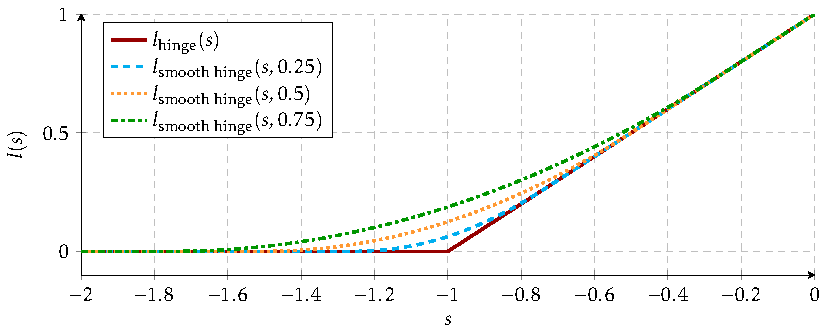
\includegraphics[width = \linewidth]{images/surrogates_smooth.pdf}
  \caption{Comparison of the hinge loss and its smoothened version with~$\varepsilon = 0.25,$~$\varepsilon = 0.5,$ and~$\varepsilon = 0.75.$}
  \label{fig: surrogates smooth}
\end{figure}

\sgd*

\pagebreak

\begin{proof}[Proof of Theorem~\ref{thm:sgd} on page~\pageref{thm:sgd}]
  We intend to apply Theorem~\ref{thm:convergence} and thus, we need to verify its assumptions. Recall the form of the objective function
  \begin{equation*}
    L(\bm{w}^k)
      = \norm{\bm{w}^k}^2 + \frac{1}{\npos} \sum_{i \in \Ipos} l(t(\bm{w}^k) - \bm{x}_i^{\top} \bm{w}^k).
  \end{equation*}
  The objective is a combination of squared norm of weights, which is strictly convex function, and a surrogate approximation of false-negative rate, which is convex function due to Theorem~\ref{thm: convexity}. Therefore, the objective~$L$ is a strictly convex function. Moreover, it is also differentiable due to Theorem~\ref{thm: differentiability} and differentiability of smoothened hinge loss~$l$. As a result, Assumption~\ref{ass_convex} is satisfied.

  Lemma~\ref{lemma:bound_g} says that~$\norm{g(\bm{w}^k)} \leq \norm{\bm{w}^k} + \hat{B}$ for all~$k.$ To show that Assumption~\ref{ass_gbound} is satisfied, we have to show, that~$\norm{\bm{w}^k}$ is uniformly bounded. Consider sufficiently large~$k$ such that~$\alpha^k < 1.$ Then
  \begin{align*}
    \norm{\bm{w}^{k+1}}
      & = \norm{\bm{w}^{k} - \alpha^k g(\bm{w}^{k})}
        = \norm{(1 - \alpha^k)\bm{w}^{k} - \alpha^k \frac{1}{\nmbpos^k} \sum_{i \in \Imbpos^k} l'(t^k - s_i^k)(\nabla t^k - \bm{x}_i)} \\
      & \leq (1 - \alpha^k) \norm{\bm{w}^{k}} + \alpha^k \norm{\frac{1}{\nmbpos^k} \sum_{i \in \Imbpos^k} l'(t^k - s_i^k)(\nabla t^k - \bm{x}_i)}
      \leq (1 - \alpha^k) \norm{\bm{w}^{k}} + \alpha^k \hat{B},
  \end{align*}
  where the first inequality follows from the triangle inequality and the last from the proof of Lemma~\ref{lemma:bound_g}. Now we have two possible cases
  \begin{itemize}
    \item If $\norm{\bm{w}^k} \leq \hat{B},$ then we get
    \begin{equation*}
      \norm{\bm{w}^{k+1}}
        \leq (1 - \alpha^k) \norm{\bm{w}^{k}} + \alpha^k \hat{B}
        \leq (1 - \alpha^k) \hat{B} + \alpha^k \hat{B}
        = \hat{B}.
    \end{equation*}
    \item If $\norm{\bm{w}^k} > \hat{B},$ then we get
    \begin{equation*}
      \norm{\bm{w}^{k+1}}
        \leq (1 - \alpha^k) \norm{\bm{w}^{k}} + \alpha^k B
        < (1 - \alpha^k) \norm{\bm{w}^{k}} + \alpha^k \norm{\bm{w}^{k}}
        = \norm{\bm{w}^{k}}.
    \end{equation*}
  \end{itemize}
  Therefore, for sufficiently large~$k,$ we have~$\norm{\bm{w}^{k}} \leq \max \Brac[c]{\hat{B}, \; \norm{\bm{w}^0}}.$ Combining this with Lemma~\ref{lemma:bound_g}, we get~$\norm{g(\bm{w}^k)} \leq B,$ for some~$B,$ and Assumption~\ref{ass_gbound} is satisfied.

  Assumptions~\ref{ass_alpha1}-\ref{ass_alpha3} are imposed directly in the statement of this theorem. 

  It remains to verify~\eqref{eq:nec_cond}. For simplicity, we will do so only for~$\vartheta = 1$ and for~$2$ minibatches of the same size. However, the proof would be identical for different~$\vartheta$ and more minibatches. From the assumptions, we have two minibatches~$\Imb^k$ and~$\Imb^{k+1}$, which are pairwise disjoint and cover all samples. Moreover, for all~$k,$ we have~$\Imb^k = \Imb^{k+2}.$ Furthermore, the assumptions imply that the number of positive samples in each minibatch is equal to~$\nmbpos^k = \frac{1}{2} \npos$, where~$\npos$ is the total number of positive samples.
   
   First we estimate the difference between~$s_i^k$ defined in~\eqref{eq:defin_z} and~$\bm{x}_i^\top \bm{w}^k$. For any~$i \in \Imb^k$ we have~$s_i^k = \bm{x}_i^\top \bm{w}^k.$ Since we have two disjoint minibatches, due to the construction~\eqref{eq:defin_z} we get
  \begin{equation}\label{eq:sgd_estimate_z1}
    \begin{aligned}
      s_i^{k-1}
        & = s_i^{k-2}
          = \bm{x}_i^\top \bm{w}^{k-2}
          = \bm{x}_i^\top \Brac{\bm{w}^k + \alpha^{k-2}g(\bm{w}^{k-2}) + \alpha^{k-1} g(\bm{w}^{k-1})} \\
        & = \bm{x}_i^\top \bm{w}^k + \alpha^{k-2}\bm{x}_i^\top g(\bm{w}^{k-2}) + \alpha^{k-1}\bm{x}_i^\top g(\bm{w}^{k-1}).
    \end{aligned}
  \end{equation}
  Similarly, due to the construction of~$s_i^k$ from~\eqref{eq:defin_z}, we have for~$i \notin \Imb^k$
  \begin{equation}\label{eq:sgd_estimate_z2}
    s_i^k
    = s_i^{k-1}
    = \bm{x}_i^\top \bm{w}^{k-1}
    = \bm{x}_i^\top (\bm{w}^k+\alpha^{k-1}g(\bm{w}^{k-1}))
    = \bm{x}_i^\top \bm{w}^k + \alpha^{k-1}\bm{x}_i^\top g(\bm{w}^{k-1}).
  \end{equation}
  Recall that we already verified~\ref{ass_convex}-\ref{ass_alpha3}. Combining~\ref{ass_gbound} with~\eqref{eq:sgd_estimate_z1} and~\eqref{eq:sgd_estimate_z2} yields the existence of some~$C_2$ such that for all~$i \in \I$ we have
  \begin{equation}\label{eq:estimate_diff_z}
    \begin{aligned}
      \norm{s_i^k - \bm{x}_i^\top \bm{w}^k} &\leq C_2\alpha^{k-1}, \quad & \quad 
      \norm{s_i^{k-1} - \bm{x}_i^\top \bm{w}^k} &\leq C_2\Brac{\alpha^{k-1}+\alpha^{k-2}}.
    \end{aligned}
  \end{equation}
  This also immediately implies
  \begin{equation}\label{eq:estimate_diff_t}
    \begin{aligned}
      \norm{t^k - t(\bm{w}^k)}     & \leq C_2\alpha^{k-1}, \quad & \quad
      \norm{t^{k-1} - t(\bm{w}^k)} & \leq C_2\Brac{\alpha^{k-1}+\alpha^{k-2}}.
    \end{aligned}
  \end{equation}
  Moreover, we know that~$l'$ is Lipschitz continuous with Lipschitz constant~$D$ according to~\ref{surr_der2}. Then due to~\eqref{eq:estimate_diff_z} and~\eqref{eq:estimate_diff_t} we get
  \begin{equation}\label{eq:sgd_lipschitz1}
    \norm{l'(t^k-s_i^k) - l'(t(\bm{w}^k)-\bm{x}_i^\top \bm{w}^k)}
      \leq D \norm{t^k-s_i^k - t(\bm{w}^k)+ \bm{x}_i^\top \bm{w}^k}
      \leq  2C_2 D \alpha^{k-1}.
  \end{equation}
  In an identical way, we can derive the following relations
  \begin{equation}\label{eq:sgd_lipschitz2}
    \begin{aligned}
      \norm{l'(t^{k-1}-s_i^{k-1}) - l'(t(\bm{w}^k)-\bm{x}_i^\top \bm{w}^k)}
        & \leq 2C_2D\Brac{\alpha^{k-1}+\alpha^{k-2}}, \\
      \norm{l'(s_i^k-t^k) - l'(\bm{x}_i^\top \bm{w}^k-t(\bm{w}^k))}
        & \leq 2C_2D\alpha^{k-1}, \\
      \norm{l'(s_i^{k-1}-t^{k-1}) - l'(\bm{x}_i^\top \bm{w}^k-t(\bm{w}^k))}
        & \leq 2C_2D\Brac{\alpha^{k-1}+\alpha^{k-2}}.
    \end{aligned}
  \end{equation}
  Now we need to estimate the distance between~$\nabla t(\bm{w}^k)$ and~$\nabla t^k$. By plugging~\eqref{eq:update_a} into~\eqref{eq:update_nablat}, we get
  \begin{equation*}
    \nabla t^k
      = \frac{\sum_{i \in \Imb^k} l'(s_i^k - t^k)\bm{x}_i + \sum_{i \in \Imb^{k-1}} l'(s_i^{k-1} - t^{k-1}) \bm{x}_i}{\sum_{i \in \I} l'(s_i^k - t^k)}.
  \end{equation*}
  Moreover, using Theorem~\ref{thm: differentiability} and the fact that we have only two minibatches and therefore for any~$k$ we have~$\I = \Imb^k \cup \Imb^{k-1}$, we get
  \begin{equation*}
    \nabla t(\bm{w}^k)
      = \frac{\sum_{i \in \Imb^k} l'(\bm{x}_i^\top \bm{w}^k - t(\bm{w}^k))\bm{x}_i + \sum_{i \in \Imb^{k-1}} l'(\bm{x}_i^\top \bm{w}^k - t(\bm{w}^k))\bm{x}_i}{\sum_{i \in \I} l'(\bm{x}_i^\top \bm{w}^k - t(\bm{w}^k))}.
  \end{equation*}
  From Lemma~\ref{lemma:bound_zero} we deduce that the denominators in the relations above are bounded away from zero uniformly in~$k$. Assumption~\ref{ass_alpha2} implies ~$\alpha^k \to 0$. This allows us to use Lemma~\ref{lemma:ratio} which together with~\eqref{eq:sgd_lipschitz2} implies that there is some~$C_3$ such that for all sufficiently large~$k$ we have
  \begin{equation}\label{eq:sgd_nablat_diff}
    \norm{\nabla t^k - \nabla t(\bm{w}^k)} \leq C_3\Brac{\alpha^{k-1} + \alpha^{k-2}}.
  \end{equation}
  Using the assumptions above, we can simplify the terms for~$g(\bm{w}^k)$ from~\eqref{eq:update_g} and~$\nabla L(\bm{w}^k)$ from~\eqref{eq:derivatives} to
  \begin{equation*}
    \begin{aligned}
      g(\bm{w}^k)
        & = \bm{w}^{k} + \frac{2}{\npos} \sum_{i \in \Imbpos^k} l'(t^k - s_i^k)(\nabla t^k - \bm{x}_i), \\
      g(\bm{w}^{k+1})
        & = \bm{w}^{k+1} + \frac{2}{\npos} \sum_{i \in \Imbpos^{k+1}} l'(t^{k+1}-s_i^{k+1})(\nabla t^{k+1} - \bm{x}_i), \\
      \nabla L(\bm{w}^k)
        & = \bm{w}^{k} + \frac{1}{\npos} \sum_{i \in \Ipos} l'(t(\bm{w}^k) - \bm{x}_i^\top \bm{w}^k)(\nabla t(\bm{w}^k) - \bm{x}_i), \\
      \nabla L(\bm{w}^{k+1})
        & = \bm{w}^{k+1} + \frac{1}{\npos} \sum_{i \in \Ipos} l'(t(\bm{w}^{k+1}) - \bm{x}_i^\top \bm{w}^{k+1})(\nabla t(\bm{w}^{k+1}) - \bm{x}_i).
    \end{aligned}
  \end{equation*}
  Due to the assumptions, we have~$\Ipos = \Imbpos^k \cup \Imbpos^{k+1}$ and~$\emptyset = \Imbpos^k \cap \Imbpos^{k+1}$, which allows us to write
  \begin{subequations}\label{eq:sgd_sum}
    \begin{align}
    \label{eq:sgd_sum1}
    \npos & \Brac{g(\bm{w}^k) + g(\bm{w}^{k+1}) - \nabla L(\bm{w}^k)-\nabla L(\bm{w}^{k+1})}\\
    \label{eq:sgd_sum2}
    & = \sum_{i \in \Imbpos^k} l'(t^k - s_i^k)(\nabla t^k - \bm{x}_i) - \sum_{i \in \Imbpos^k} l'(t(\bm{w}^k) - \bm{x}_i^\top \bm{w}^k)(\nabla t(\bm{w}^k) - \bm{x}_i) \\
    \label{eq:sgd_sum3}
    & + \sum_{i \in \Imbpos^k} l'(t^k - s_i^k)(\nabla t^k - \bm{x}_i) - \sum_{i \in \Imbpos^k} l'(t(\bm{w}^{k+1}) - \bm{x}_i^\top \bm{w}^{k+1})(\nabla t(\bm{w}^{k+1}) - \bm{x}_i)\\
    \label{eq:sgd_sum4}
    & + \sum_{i \in \Imbpos^{k+1}} l'(t^{k+1} - s_i^{k+1})(\nabla t^{k+1} - \bm{x}_i) - \sum_{i\in \Imbpos^{k+1}}l'(t(\bm{w}^k) - \bm{x}_i^\top \bm{w}^k)(\nabla t(\bm{w}^k) - \bm{x}_i) \\
    \label{eq:sgd_sum5}
    & + \sum_{i \in \Imbpos^{k+1}} l'(t^{k+1} - s_i^{k+1})(\nabla t^{k+1} - \bm{x}_i)  - \sum_{i \in \Imbpos^{k+1}} l'(t(\bm{w}^{k+1}) - \bm{x}_i^\top \bm{w}^{k+1})(\nabla t(\bm{w}^{k+1}) - \bm{x}_i).
    \end{align}
  \end{subequations}
  Then relations~\eqref{eq:sgd_lipschitz1} and~\eqref{eq:sgd_nablat_diff} applied to Lemma~\ref{lemma:product} imply
  \begin{equation*}
    \norm{\sum_{i \in \Imbpos^k} l'(t^k - s_i^k)(\nabla t^k - \bm{x}_i) - \sum_{i \in \Imbpos^k} l'(t(\bm{w}^k) - \bm{x}_i^\top \bm{w}^k)(\nabla t(\bm{w}^k) - \bm{x}_i)} \leq C_4 \Brac{\alpha^{k-1} + \alpha^{k-2}}
  \end{equation*}
  for some~$C_4$, which gives a bound for~\eqref{eq:sgd_sum2}. Bound for~\eqref{eq:sgd_sum5} is obtained by increasing~$k$ by one. Bounds for~\eqref{eq:sgd_sum3} and~\eqref{eq:sgd_sum4} can be find similarly using~\eqref{eq:sgd_lipschitz2}. Altogether, we showed
  \begin{equation}\label{eq:nec_cond3}
    \norm{g(\bm{w}^k) + g(\bm{w}^{k+1}) - \nabla L(\bm{w}^k) - \nabla L(\bm{w}^{k+1})}
      \leq C_1(\alpha^{k-2} + \alpha^{k-1} + \alpha^{k} + \alpha^{k+1})
  \end{equation}
  for some~$C_1$.
  
  We now estimate
  \begin{equation}\label{eq:proof_est1}
    \begin{aligned}
      \alpha^k
      & \inner{ g(\bm{w}^{k})-\nabla L(\bm{w}^{k})}{\bm{w}^*-\bm{w}^{k}} + \alpha^{k+1}\inner{ g(\bm{w}^{k+1})-\nabla L(\bm{w}^{k+1})}{\bm{w}^*-\bm{w}^{k+1}} \\
      & = \inner{ g(\bm{w}^{k})-\nabla L(\bm{w}^{k})}{\alpha^k(\bm{w}^*-\bm{w}^{k})}
        + \inner{ g(\bm{w}^{k+1})-\nabla L(\bm{w}^{k+1})}{\alpha^{k+1}(\bm{w}^*-\bm{w}^{k+1})} \\
      & = \inner{ g(\bm{w}^{k})-\nabla L(\bm{w}^{k}) + g(\bm{w}^{k+1})-\nabla L(\bm{w}^{k+1})}{\alpha^k(\bm{w}^*-\bm{w}^{k})} \\
      & + \inner{ g(\bm{w}^{k+1})-\nabla L(\bm{w}^{k+1})}{\alpha^{k+1}(\bm{w}^*-\bm{w}^{k+1})-\alpha^k(\bm{w}^*-\bm{w}^{k})}.
    \end{aligned}
  \end{equation}
  To estimate the second part of the right hand side of~\eqref{eq:proof_est1}, we make use of Lemma~\ref{lemma:bound_g} to obtain the existence of some~$C_5$ such that
  \begin{equation}\label{eq:proof_est2}
    \begin{aligned}
    & \inner{ g(\bm{w}^{k+1})
    -\nabla L(\bm{w}^{k+1})}{\alpha^{k+1}(\bm{w}^*-\bm{w}^{k+1})-\alpha^k(\bm{w}^*-\bm{w}^{k})} \\
    & \leq 2B\norm{\alpha^{k+1}(\bm{w}^*-\bm{w}^{k+1})-\alpha^k(\bm{w}^*-\bm{w}^{k})} \\
    & = 2B\norm{\alpha^{k+1}(\bm{w}^*-\bm{w}^k+\alpha^kg(\bm{w}^k))-\alpha^k(\bm{w}^*-\bm{w}^{k})} \\
    & = 2B\norm{(\alpha^{k+1}-\alpha^k)\bm{w}^* + (\alpha^k-\alpha^{k+1})\bm{w}^k + \alpha^k\alpha^{k+1} g(\bm{w}^k)} \\
    & \leq C_5 \norm{\alpha^{k+1}-\alpha^k} + C_5(\alpha^k)^2 + C_5(\alpha^{k+1})^2.
    \end{aligned}
  \end{equation}
  In the last inequality we used the inequality~$2ab\leq a^2+b^2$. To estimate the first part of the right hand side of~\eqref{eq:proof_est1}, we can apply~\eqref{eq:nec_cond3} together with the boundedness of~$\{\bm{w}^k\}$ to obtain the existence of some~$C_6$ such that
  \begin{equation}\label{eq:proof_est3}
    \begin{aligned}
    \inner{ g(\bm{w}^{k}) -\nabla L(\bm{w}^{k}) + g(\bm{w}^{k+1})-\nabla L(\bm{w}^{k+1})}{\alpha^k(\bm{w}^* - \bm{w}^{k})} \\
      \leq C_6(\alpha^{k-2})^2 + C_6(\alpha^{k-1})^2 + C_6(\alpha^{k})^2 + C_6(\alpha^{k+1})^2.
      \end{aligned}
  \end{equation}
  Plugging~\eqref{eq:proof_est2} and~\eqref{eq:proof_est3} into~\eqref{eq:proof_est1} and summing the terms yields~\eqref{eq:nec_cond}. Then the assumptions of Theorem~\ref{thm:convergence} are verified and the theorem statement follows.
\end{proof}

\subsection{Auxiliary Results}\label{app:sgd3}

\begin{lemma}\label{lemma:bound_zero}
  Let~$l$ satisfy~\ref{surr_basic1}-\ref{surr_ratio}. Then there exists some~$\hat{C} > 0$ such that for all~$k$ we have
  \begin{align*}
    \hat{C} \leq & \sum_{i \in \I} l'(s_i^k - t^k), \quad & \quad
    \hat{C} \leq & \sum_{i \in \I} l'(\bm{x}_i^\top \bm{w}^k - t(\bm{w}^k)).
  \end{align*}
\end{lemma}
\begin{proof}
  First, we will find an upper bound of~$s_i^k-t^k$. Fix any index~$i_0$. Since~$l$ is nonnegative due to~\ref{surr_basic1}, equation~\eqref{eq:update_t} implies
  \begin{equation*}
    n\tau = \sum_{i \in \I} l(s_i^k - t^k) \geq l(s_{i_0}^k - t^k).
  \end{equation*}
  Since~$l$ is a strictly increasing function due to~\ref{surr_basic2} and~$n\tau>0$, we get 
  \begin{equation}\label{eq:sigma_bound}
    l^{-1}(n\tau) \geq s_{i_0}^k-t^k.
  \end{equation}
  Since~$i_0$ was an arbitrary index, it holds true for all indices. Then~\ref{surr_ratio} which leads to a further estimate
  \begin{equation*}
    \sum_{i \in \I} l'(s_i^k - t^k)
      = \sum_{i\in \I} l(s_i^k-t^k) \frac{l'(s_i^k-t^k)}{l(s_i^k-t^k)}
      \geq \sum_{i \in \I} l(s_i^k - t^k) \frac{l'(l^{-1}(n\tau))}{l(l^{-1}(n\tau))}
      = n\tau \frac{l'(l^{-1}(n\tau))}{l(l^{-1}(n\tau))}
      = l'(l^{-1}(n\tau)),
  \end{equation*}
  where the inequality follows from~\eqref{eq:sigma_bound} and the following equality from~\eqref{eq:update_t}. Due to~\ref{surr_basic2} we obtain that~$l'(l^{-1}(n\tau))$ is a positive number, which finishes the proof of the first part. The second part can be obtained in an identical way.
\end{proof}

\pagebreak

\begin{lemma}\label{lemma:bound_g}
  Let~$l$ satisfy~\ref{surr_basic1}-\ref{surr_der1}. Then there exists some~$\hat{B}$ such that for all~$k$ we have
  \begin{equation*}
    \begin{aligned}
      \norm{\nabla L(\bm{w}^k)} & \leq \norm{\bm{w}^k} +  \hat{B}, \quad & \quad
      \norm{g(\bm{w}^k)} & \leq \norm{\bm{w}^k} + \hat{B}.
    \end{aligned}
  \end{equation*}
\end{lemma}
\begin{proof}
  By applying norm to the gradient~\eqref{eq:derivatives} of the objective function~$L,$ we get 
  \begin{equation*}
    \norm{\nabla L(\bm{w}^k)}
      \leq \norm{\bm{w}^k} + \norm{\frac{1}{\npos} \sum_{i \in \Ipos} l'(t(\bm{w}^k) - \bm{x}_i^{\top} \bm{w}^k)(\nabla t(\bm{w}^k) - \bm{x}_i)},
  \end{equation*}
  where the inequality follows from the triangle inequality. Due to~\ref{surr_der1} the derivative~$l'$ is bounded by some~$\hat{C}_1$. Then Theorem~\ref{thm: differentiability} and Lemma~\ref{lemma:bound_zero} imply
  \begin{equation*}
    \norm{\nabla t(\bm{w}^k)}
      \leq \frac{\hat{C}_1 \sum_{i \in \I} \norm{\bm{x}_i}}{\sum_{i \in \I} l'(\bm{x}_i^\top \bm{w}^k - t(\bm{w}^k))}
      \leq \frac{\hat{C}_1}{\hat{C}_2} \sum_{i\in \I} \norm{\bm{x}_i},
  \end{equation*}
  which is independent of~$k$. Then~\eqref{eq:derivatives} and again the boundedness of~$l'$ imply the existence of some~$\hat{B}$ such that~$\norm{\nabla L(\bm{w}^k)} \leq \norm{\bm{w}^k} + \hat{B}$ for all~$k$. The proof for~$g(\bm{w}^k)$ can be performed identically.
\end{proof}

\begin{lemma}\label{lemma:ratio}
  Consider uniformly bounded positive sequences~$c_1^k,$~$c_2^k,$~$d_1^k,$~$d_2^k,$~$\alpha^k$ and positive constants $C_1$, $C_2$ such that for all~$k$ we have
  \begin{equation*}
    \begin{aligned}
      \norm{c_1^k-c_2^k} & \leq C_1\alpha^k, \quad &
      \norm{d_1^k-d_2^k} & \leq C_1\alpha^k, \quad &
      d_1^k & \geq C_2, \quad &
      d_2^k & \geq C_2.
    \end{aligned}
  \end{equation*}
  If~$\alpha^k \to 0$, then there exists a constant~$C_3$ such that for all sufficiently large~$k$ we have
  \begin{equation*}
    \norm{\frac{c_1^k}{d_1^k} - \frac{c_2^k}{d_2^k}} \leq C_3\alpha^k.
  \end{equation*}
\end{lemma}

\begin{proof}
  Since~$d_1^k$ and~$d_2^k$ are bounded away from zero and since~$\alpha^k \to 0$, we have
  \begin{equation*}
    \norm{\frac{c_1^k}{d_1^k} - \frac{c_2^k}{d_2^k}}
      \leq \max\Brac[c]{\frac{c_1^k}{d_1^k} - \frac{c_1^k+C_1\alpha^k}{d_1^k-C_1\alpha^k}, \; \frac{c_1^k}{d_1^k} - \frac{c_1^k-C_1\alpha^k}{d_1^k+C_1\alpha^k}}.
  \end{equation*}
  The first term can be estimated as
  \begin{equation*}
    \norm{\frac{c_1^k}{d_1^k} - \frac{c_1^k+C_1\alpha^k}{d_1^k-C_1\alpha^k}}
    = \norm{\frac{(c_1^k+d_1^k)C_1\alpha^k}{d_1^k(d_1^k-C_1\alpha^k)}}
    \leq \frac{(c_1^k+d_1^k)C_1\alpha^k}{C_2|d_1^k-C_1\alpha^k|}.
  \end{equation*}
  Since~$\alpha^k\to 0$ by assumption, for large~$k$ we have~$\norm{d_1^k-C_1\alpha^k}\geq \frac{1}{2}C_2$. Since the sequences are uniformly bounded, the statement follows.
\end{proof}

\pagebreak

\begin{lemma}\label{lemma:product}
  Consider scalars~$a_i,$~$c_i$ and vectors~$b_i,$~$d_i.$ If there is some~$\hat{C}$ such that~$\abs{a_i} \leq \hat{C}$ and~$\norm{d_i} \leq \hat{C}$, then
  \begin{equation*}
    \norm{\sum_{i=1}^n a_ib_i - \sum_{i=1}^n c_id_i}
      \leq \hat{C}\sum_{i=1}^n \Brac{\abs{a_i-c_i} + \norm{b_i-d_i}}.
  \end{equation*}
\end{lemma}

\begin{proof}
  It is simple to verify
  \begin{equation*}
    \norm{\sum_{i=1}^n a_ib_i - \sum_{i=1}^n c_id_i} \leq \sum_{i=1}^n \norm{d_i}\abs{a_i-c_i} + \sum_{i=1}^n \abs{a_i}\norm{b_i-d_i},
  \end{equation*}
  from which the statement follows.
\end{proof}

\newpage
